\documentclass[preprint]{acm_proc_article-sp}
\usepackage{graphicx}
\DeclareGraphicsExtensions{.jpg,.jpeg}
\renewcommand{\baselinestretch}{1.0}
\begin{document}
\newcommand{\tmark}{^{\mbox{TM}}}
\title{The GridPACK$\tmark$ Toolkit for Developing Power Grid Simulations on High
Performance Computing Platforms}

\numberofauthors{9}
\author{
\alignauthor
Bruce Palmer
\affaddr{Pacific Northwest National Laboratory}
\affaddr{Richland, WA 99352}
\affaddr{bruce.palmer@pnnl.gov}
\alignauthor
William Perkins
\affaddr{Pacific Northwest National Laboratory}
\affaddr{Richland, WA 99352}
\affaddr{william.perkins@pnnl.gov}
\alignauthor
Kevin Glass
\affaddr{Pacific Northwest National Laboratory}
\affaddr{Richland, WA 99352}
\affaddr{kevin.glass@pnnl.gov}
\and
\alignauthor
Yousu Chen
\affaddr{Pacific Northwest National Laboratory}
\affaddr{Seattle, WA}
\affaddr{yousu.chen@pnnl.gov}
\alignauthor
Shuangshuang Jin
\affaddr{Pacific Northwest National Laboratory}
\affaddr{Seattle, WA}
\affaddr{shuangshuang.jin@pnnl.gov}
\alignauthor
David Callahan
\affaddr{Northwest Institute for Advanced Computing}
\affaddr{Seattle, WA}
\affaddr{david.callahan@pnnl.gov}
}
\additionalauthors{
Mark Rice \\
Pacific Northwest National Laboratory\\
Richland, WA 99352 \\
mark.rice@pnnl.gov \\
\\
Ruisheng Diao\\
Pacific Northwest National Laboratory\\
Richland, WA 99352 \\
ruisheng.diao@pnnl.gov\\
\\
Stephen Elbert \\
Pacific Northwest National Laboratory\\
Richland, WA 99352 \\
stephen.elbert@pnnl.gov\\
\\
Zhenyu (Henry) Huang \\
Pacific Northwest National Laboratory \\
Richland, WA 99352 \\
zhenyu.huang@pnnl.gov \\
}

\toappear{\copyright 2013 Association for Computing Machinery. ACM
acknowledges that this contribution was authored or co-authored by an employee,
contractor or affiliate of the United States Government. As such, the United
States Government retains a nonexclusive, royalty-free right to publish or
reproduce this article, or to allow others to do so, for Government purposes
only. HiPCNA-PG '13, November 17-21 2013, Denver, CO, USA Copyright 2013 ACM
978-1-4053-2510-3/13/11.\$15.00. http://dx.doi.org/10.1145/2536780.2536782}

\maketitle
\begin{abstract}
This paper describes the GridPACK\texttrademark framework, which is designed to help
power grid engineers develop modeling software capable of running on high
performance computers. The framework contains modules for setting up distributed
power grid networks, assigning buses and branches with arbitrary behaviors to
the network, creating distributed matrices and vectors, using parallel linear
and non-linear solvers to solve algebraic equations, and mapping functionality
to create matrices and vectors based on properties of the network. In addition,
the framework contains additional functionality to support IO and to manage
errors. The goal of GridPACK\texttrademark is to provide developers with a
comprehensive set of modules that can substantially reduce the complexity of
writing software for parallel computers
while still providing efficient and scalable software solutions.
\end{abstract}

\keywords{Electric Power Grid, High Performance Computing, Software Frameworks}

\section{Introduction}
The electric power grid has been characterized as being the largest machine in
the world, but in spite of this it is still being modeled primarily on workstations running
serial programs. Much smaller systems (e.g. the internal combustion engine\cite{EXACT}),
on the other hand, are being modeled in ways that can fully exhaust the resources of
the largest available computing systems. Power grid engineers have spent
enormous effort and ingenuity reducing simulations of the grid to manageable sizes,
but these reductions have resulted in approximations and loss of detail which may
be hiding or obscuring important features and behaviors of the power network.
Furthermore, as the
power grid becomes more complicated, due to more varied and unpredictable energy sources
such as wind and solar energy and the influx of more information from data sources
such as smart
meters, the task of modeling even small networks becomes more challenging. The
power grid is clearly an appealing target for high performance computing (HPC)
but there are few
tools available to assist power grid engineers interested in writing code to run on
HPC platforms.

This paper will describe the GridPACK\texttrademark framework for developing parallel
power grid simulations that run on HPC platforms with high levels of
performance and scalability. Frameworks have appeared in other contexts and been
used to reduce the programming burden on domain scientists by making complex
but commonly used motifs available through libraries or other mechanisms.
Both the Community Climate System Model\cite{CCSM} and Weather Research
and Forecasting Model\cite{WRF} are framework-based
approaches to developing climate and weather models. The Cactus framework is
designed to support grid-based applications and is widely used in the numerical
general relativity community\cite{CACTUS}. The Common Component
Architecture\cite{CCA} is a framework
designed to support modularization of codes and has been used successfully in
some groundwater applications\cite{SPH}. Other examples of frameworks or modular approaches
to code development can be found, particularly among large software projects
with a broad developer base.

The GridPACK\texttrademark toolkit is designed to allow power
system engineers to focus on developing working applications from their
models without getting bogged down in the details of decomposing the computation
across multiple processors, managing data transfers between processors, working out
index transformations between power grid networks and the matrices generated by
different power applications, and managing input and output.
GridPACK\texttrademark encapsulates as much of the book-keeping required to set up HPC
applications as possible in high-level programming abstractions that allow developers
to concentrate on the physics and mathematics of their problems.
The following will summarize the overall design of the GridPACK\texttrademark
framework and then
describe the major modules that have been developed so far.
%We will briefly
%discuss how these can be integrated together to create a working application.

\newpage
\section{Power Grid Requirements}
The initial focus of the GridPACK\texttrademark design analysis was to target
four power grid
applications and to identify common features that span multiple applications.
This analysis included a breakdown of the
application into phases and identification within each phase of the functionality
required to complete them. The four applications originally targeted within this
project were power flow simulations\cite{PF}, contingency analysis\cite{CA},
state estimation\cite{SE} and
dynamic simulation\cite{DS}. This analysis identified three major categories of
functionality that
required support from the framework and a number of smaller categories that were
extremely useful. The categories are:
\begin{itemize}
\item Distributed graphs representing the network topology of the power grid
and flexibility in specifying the behavior of objects located on the network.
The power grid network is represented as a graph with edges referred to a
branches and nodes referred to as buses. 
\item Distributed matrices and vectors and parallel solvers and
preconditioners. The solution algorithms for power grid problems are usually
expressed in terms of linear or non-linear algebraic equations. 
\item Mapping objects located on the network to distributed matrices and vectors.
For example, the diagonal elements of the admittance matrix are associated with
buses and the off-diagonal elements are associated with branches. The mapping
between the network and matrix elements can be automated to a considerable
extent.
\end{itemize}
These three areas encompose two major classes of data objects,
distributed networks and distributed matrices and vectors. One of the goals of
GridPACK\texttrademark was to create support for these data objects and transformations
between the two.

The network topology is the starting point for any power grid analysis. The
topology defines the initial network model and is the connection point between
the physical problem definition in terms of buses and branches and the solution
method, which is usually expressed in terms of matrices and vectors. Because the
network is expected to be a large data object, it is undesirable to replicate
it across processors. Instead, the network is divided across processors
to both minimize the memory utilization on each process and to minimize
communication volume between processors. The GridPACK\texttrademark framework needs to
support the distribution of the network along with the exchange of data that is
required between processors. Data exchanges are required because parts of the
network located on one processor need to access the buses and branches they are
attached to that reside on other processors. This is particularly true for
problems that rely on an iterative loop for their solution where network
exchanges need to occur at each iteration.

The network also serves as a container for the objects that define the behavior
of buses and branches in the actual power grid model. These objects represent
the physical system being modeled as well as the analyses that are being
performed on it. All the things that might be present on a bus or branch,
such as generators, loads, grounds, transformers, sensors, etc. need to be
contained within the bus and branch objects. Bus and branch behaviors frequently
depend on the objects immediately attached to them so that buses depend on the
branches that are attached to them (and possibly on the buses attached to them
via a branch) and branches depend on the buses attached at either end of the
branch. Providing easy access to these attached objects is another function of the
network module.

Basic algebraic objects, such as matrices and vectors, are a core part
of the solution algorithms required by power grid analyses. These also tend to
be large data objects that must be distributed across processors. Furthermore,
the solution algorithms built around these data objects are generally the most
time consuming part of program execution, so it is necessary to ensure that the
solutions are fully parallel as well. Most solution algorithms
are dominated by sparse matrices but a few, such as Kalman filter
analyses\cite{KAL}, require dense
matrices. Vectors are typically dense. There exists a rich set of libraries for
constructing distributed matrices and vectors and these also contain preconditioner
and solver capabilities.  GridPACK\texttrademark leverages this work heavily by
creating wrappers
around these libraries to create matrices and vectors that can be used in solution
algorithms. Wrapping these libraries instead of using them directly has the
advantage that creating these algebraic objects can be simplified somewhat for power grid
applications but more importantly, it allows developers to investigate new
solver and algebraic libraries seamlessly, without disrupting other parts of the code.
The current GridPACK\texttrademark implementation is built on top of the
PETSc\cite{PETSC}
libraries but other possibilities include Hypre\cite{HYPRE} and
Trilinos\cite{TRIL}. All these
libraries support distributed matrices and vectors, basic algebraic operations
such matrix-vector multiply, inner products, etc. and a variety of solution
methods for linear and non-linear equations.

Finally, there is a need to support generation of matrices from objects in the
network and the ability to push data from solution vectors back down into
network objects. This is one of the most complicated and error-prone parts of
writing code, especially for parallel platforms. Much of the work involved in
setting up matrices can be eliminated by having users implement a few functions
that provide individual matrix elements contributed by each bus or branch. The
mapping function can then assemble these elements into a complete matrix for the
entire system. The fact that developers can focus on writing code for individual
matrix elements reduces the amount of programming required and fits in more
intuitively with the physical models. The complicated index calculations
required to evaluate global offsets that are needed to set up a distributed
matrix can be left to the framework.

\section{GridPACK\texttrademark}
This section will describe the core components identified so far and the functionality they
will support. It will start off with two components that directly support the major
underlying data objects, the power grid network and its associated data fields and matrices
and vectors. Additional components are then built on top of these (or at least in
conjunction with them). These include a partitioner to divide the network among
processors, network components that describe the physics of the different network
models and/or
analyses, factories that initialize network components and manage interactions
between the components and the network itself, mappers that
convert the current state of the network components into matrices and vectors,
solvers that supply the preconditioner and solver
functionality necessary to implement solution algorithms and input and output modules that
allow developers to import and export data using standard formats.
GridPACK\texttrademark is currently implemented as a C++ library and is designed
to be run on Linux platforms (the standard OS for most HPC architectures).
The library currently has no interface for Windows-based computers, but we
believe it will be possible to develop such a capability in the future if there
is a demand for it.

Many of these components rely heavily on external libraries to minimize
framework development time and to capitalize on the considerable investment in
time and expertise invested in them. By wrapping these libraries in interfaces geared
towards power grid applications they can be made easier to use by power grid
engineers. The interfaces also make it possible to swap out libraries in the future for new
or improved implementations of specific functionality without requiring application
developers to rewrite their codes. This can significantly reduce the cost of introducing
new technology into the framework and allows application specific or
vendor-proprietary algorithms to be incorporated easily into the framework.
Core framework components are described below.

\subsection{Network Module}
The network module is a templated class that can be created using any type of
model for the buses and branches. The network class has four major functions
\begin{itemize}
\item The network is a container for the network topology. The connectivity of the network
is maintained by the network object and can be made available through requests to the
network. The network also maintains the ``ghost'' status of locally held buses and
branches and determines whether a bus or branch is owned by a particular processor or
represents a ghost image of a bus or branch owned by a neighboring processor.

\item The network topology can then be decorated with bus and branch objects that reflect
the properties of the particular physical system under investigation. These bus and
branch objects are written by the application developer and model the
physical system and the analyses that need to be performed on it.
Different applications will use different bus and branch implementations.

\item The network module is responsible for implementing update operations that can be
used to fill in the value of ghost cell fields with current data from other processors.
The updates of ghost buses and ghost branches have been split into separate operations to
give users flexibility in optimizing performance by minimizing the amount of data that
needs to be communicated in the code.

\item The partitioner is responsible for distributing the network among
processors in such a way that each processor has roughly equal numbers of buses and
branches and so that buses and branches on the same processor are
mostly connected and connections to buses and branches on other processors are
minimized. This layout will optimize the communication efficiency between processors by
minimizing the number of processors that need to communicate with each other and
reducing the amount of data that must be exchanged between processors.
\end{itemize}

The combination of the functionality described above will make it possible to
build arbitrary network-based data structures and to use them in parallel
applications. The complexity of working with
the distributed network is comparable to the complexity of working with a serial
application.

\subsection{Math Module}
The math module is used to create distributed matrices and vectors and also
implements linear and non-linear solvers and their preconditioners. The math
module is designed to be a thin wrapper on top of existing parallel math
libraries. It is currently implemented using PETSc but could be implemented
using other libraries. Other implementations would not require
changes to other parts of the GridPACK\texttrademark framework or to existing
applications.

The math module consist of routines for generating distributed matrices and
vectors as well as routines for using them in linear and non-linear solvers.
Creating a matrix or vector generally consists of 1) creating the matrix or
vector object 2) adding elements to the objects using global indices and 3)
assembling the object into a state where it can be used in solvers. This
operation allows the libraries to set up internal data structures that handle
distribution of the matrix or vector and control communication
in parallel algebraic operations. Once
matrices and vectors have been created, they can be treated
as opaque objects and manipulated using a
high level API that would be comparable to writing Matlab code.

In addition to allowing user to create algebraic objects, the module
supports basic algebraic operations such as matrix-vector multiplies, scaling of
matrices and vectors, evaluation of norms, etc. The library can
also be used to create linear and non-linear solvers. Linear solvers are
can be used directly on matrices and vectors but non-linear solvers require the
creation of specific
functions that are used inside the non-linear solver to update the solutions at
each solver cycle.

\subsection{Network Components}
Network component is a generic term for objects associated with buses and branches. These
objects determine the behavior of the system and the type of analyses being done. Branch
components can represent physical objects such as transmission lines and
transformers while bus components can model loads, generators, or
something else. Both kinds of components could represent measurements (e.g.
for a state estimation analysis). 

Network components cover a broad range of behaviors and there is little that can be
said about them outside the context of a specific problem. Each component inherits from a
matrix-vector interface, which is used by the mapper module (described below) to
generate matrices and vectors. In addition, buses inherit from a base bus
interface and branches inherit from a base branch interface. These base interfaces provide
mechanisms for accessing the neighbors of a bus or branch. They also allow
developers to specify
what data is transferred in ghost exchanges. They do not define any physical
properties of
the bus or branch, it is up to application developers to do this.

The matrix-vector interface contains a set of virtual functions that must be
overwritten by the application and provide the matrix and vector elements that
define the physical model and the analyses performed on it. The type of matrix
or vector produced by a network can be changed by controlling the state of the
network components. The base bus components implements functions that can return
a list of all branches that the bus is connected to and the base branch
component can return the buses at either end of the branch. This functionality
is passed to the application by appropriately subclassing the base classes.

The class structure for the network components is shown in Figure
(\ref{classes}). 
\begin{figure}
\centering
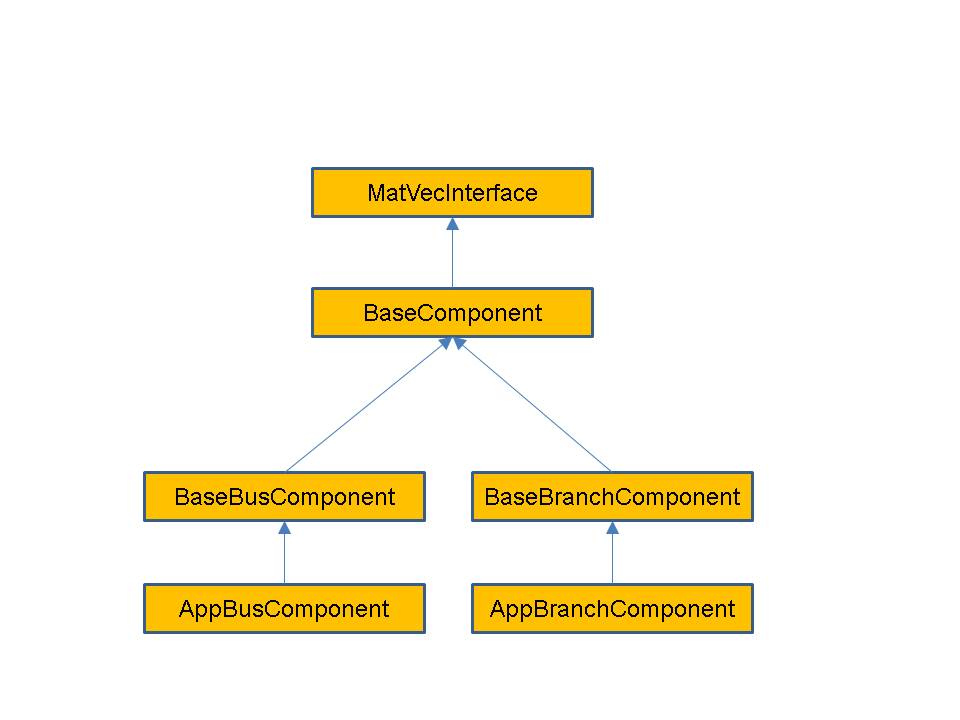
\includegraphics[width=3.5in,keepaspectratio=true]{./FigNC}
\caption{\label{classes} An inheritance diagram for the network component
classes. The base class for all network components is the MatVecInterface which
defines functions that can be overwritten by network components to produce
matrices and vectors used in computations. The BaseComponent, BaseBusComponent
and BaseBranchComponent classes define generic functions that are useful in
calculations. These include routines for obtaining neighboring buses or
branches.}
\end{figure}
Of these base classes, the MatVecInterface is the most important. It answers the
question what block of data is contributed by a bus or branch to a matrix and what
the dimensions of the block are. For example, for powerflow simulations it is
necessary to construct an entity known as the Y-matrix.  If a real-valued formulation,
the grid components on buses contribute a 2$\times$2 block to the
diagonal of the Y-matrix. Similarly, the grid components on branches contribute a 2$\times$2
block to the off-diagonal elements. If the Y-matrix is expressed as a complex
matrix, then the blocks are of size 1$\times$1. The location of these blocks in the
matrix is determined by the location of the corresponding buses and branches in the
network, but the indexing calculations required to determine this location can be made
completely transparent to the user via the mapper module. 

Because the matrix-vector interface focuses on small blocks, it is relatively easy
for power grid engineers to write the corresponding methods. The full matrices and vectors
can then be generated from the network using simple calls to the mapper interface.
For example, the equation for contributions from transmission elements on
branches to the off-diagonal elements of the Y-matrix is\cite{PF}
\begin{equation}
\label{ydiag}
Y_{branch_{mn}} = \sum_{k}\frac{-1}{r_{mnk}+jx_{mnk}}
\end{equation}
where $r_{mnk}$ is the resistance for the $k$th transmission element going from
bus $m$ to bus $n$, $x_{mnk}$ is the reactance of the $k$th transmission element
from bus $m$ to bus $n$ and $j=\sqrt{-1}$.  The sum is over the transmission
elements connecting $m$ and $n$. Information on all transmission
elements between $m$ and $n$ is already located on the $mn$ branch so this
calculation is purely local.

The contributions from buses and branches to the diagonal elements of the Y-matrix
can be written as
\begin{equation}
\label{yoffdiag}
Y_{bus_{mm}} = S_{bus_{mm}} -\sum_{n\ne m}Y_{branch_{mn}}
\end{equation}
Equation (\ref{yoffdiag}) is evaluated by looping over branches
that are connected to bus $m$. The quantities $S_{bus_{mm}}$ represent other
contributions to $Y_{bus_{mm}}$ from sources other than transmission lines.
The evaluation of these contributions is
straightforward since the BaseBusComponent and BaseBranchComponent classes already contain
methods for getting a list of all branches attached to a bus or the buses
attached to either end of a branch. The bus contribution calculation consists of
1) getting a list of the branch objects connected to the bus 2) looping over
these objects and obtaining the value of $Y_{branch_{mn}}$ from them and
3) accumulating these into $Y_{bus_{mm}}$.

The matrix-vector interface contains a number of functions that are important
for building matrices. These are divided into two sets. The first reports
back on the size of the block that the bus or branch contributes to the matrix,
the second provides the actual values in the block. To construct the Y-matrix as
a real, $2N\times 2N$ matrix, where $N$ is the number of buses in the network,
the size method for the diagonal elements (buses) and off-diagonal elements
(branches) returns the value 2 for both dimensions of the block and the values
method returns the block
\begin{equation}
\nonumber
\left[ \begin{array}{rr} a & -b \\ b & a\end{array} \right]
\end{equation}
where $a$ and $b$ the real and imaginary parts of either $Y_{bus_{mm}}$ (for
buses) or $Y_{branch_{mn}}$ (for branches). If the appropriate functions in the
matrix-vector interface have been implemented in the bus and branch components,
then matrices and vectors will automatically be built by the mapper component.
This eliminates much of the complicated detail required to evaluate global
indices when setting up a matrix.


\subsection{Mapper Module}
The mapper module contains a number of objects that can be used to generate
matrices and vectors from network components. The mappers scan the matrix-vector
interface functions in the network components and use the information provided
by them to create the corresponding matrices. The size information and the
location of the component in the network allows the mapper to calculate the
location of the element(s) in the matrix and the remaining functions provide the
actual matrix values. The matrix mapper is illustrated in Figure \ref{mapper}
for a small network.
Figure \ref{mapper}(a) shows a hypothetical network for which some buses and
branches do not contribute to the matrix as seen if Figure \ref{mapper}(b).
In addition, not all buses and branches contribute
the same size blocks. The mapping of the individual contributions from the
network in Figure \ref{mapper}(b) to initial matrix locations based on network
location is shown in Figure \ref{mapper}(c). This is followed by the elimination
of gaps in the matrix due to rows and columns with no values in Figure
\ref{mapper}(d).
\begin{figure}
\centering
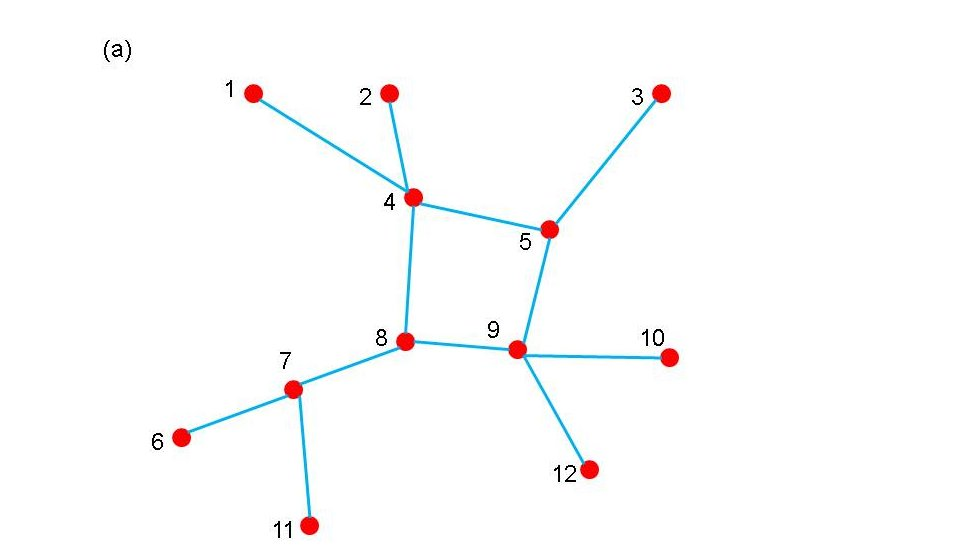
\includegraphics[width=3.5in,keepaspectratio=true]{./Fig1a}
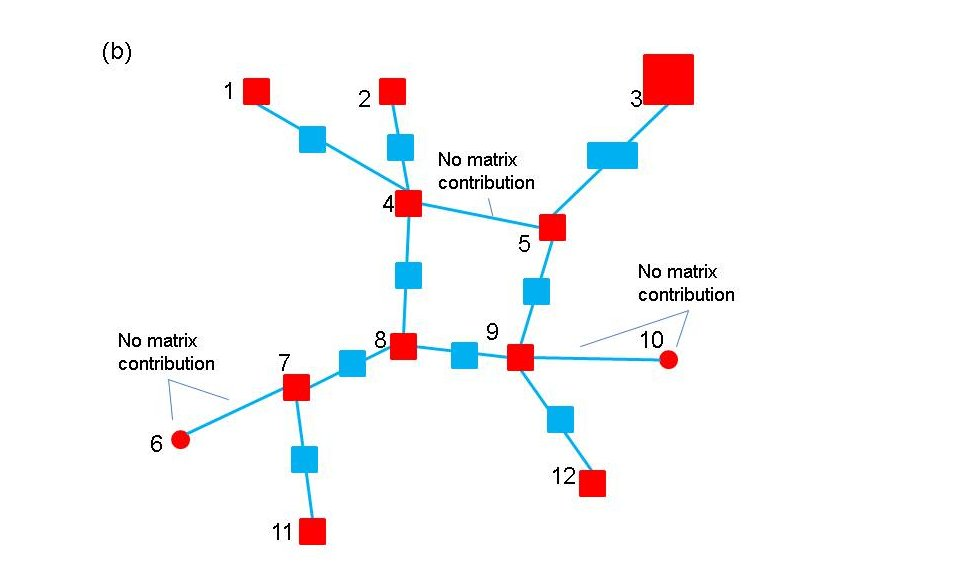
\includegraphics[width=3.5in,keepaspectratio=true]{./Fig1b}
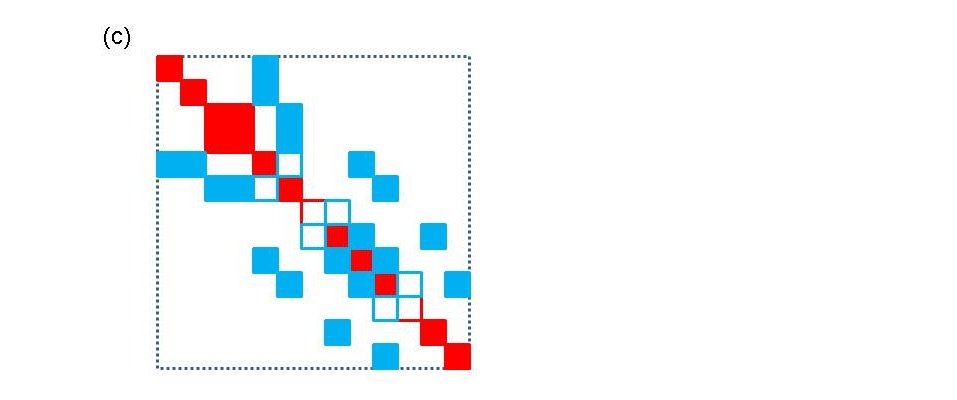
\includegraphics[width=3.5in,keepaspectratio=true]{./Fig1c}
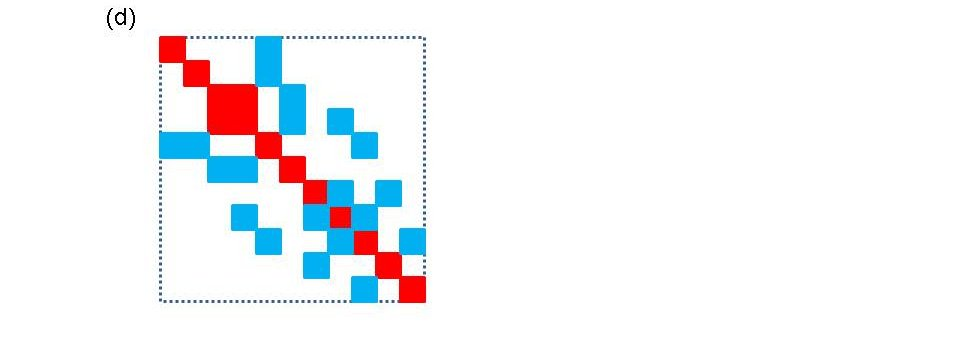
\includegraphics[width=3.5in,keepaspectratio=true]{./Fig1d}
\caption{\label{mapper} A schematic diagram of the matrix map function.
The bus numbers in (a) and (b) map to approximate column locations in (c).
(a) a small network (b)
matrix blocks associated with branches and buses. Note that not all blocks are
the same size and not all buses and branches contribute (c) initial construction
of matrix based on network indices (d) final matrix after eliminating gaps}
\end{figure}

The vector mappers are similar to the matrix mappers and are used to
construct a vector from functions
that are defined on the buses. The vector mapper can also be used to push values
from a vector back onto the buses. This is important in iterative or non-linear
solver where the matrices need to be updated based on the solutions of the
previous iteration. The solutions are first pushed back down on to the buses in the
network. The network then exchanges data between processers and based on the new
values in the buses, new matrices and vectors are produced for the next
iteration.

The matrix and vector mappers can eliminate an enormous amount of complex
programming required to set up distributed matrices and indices. In combination
with the network and math modules, it also allows developers to write code that
is fully distributed at all stages of the calculation. This will minimize memory
utilization as well as communication and redundant computation. All these are
important in developing computationally efficient and scalable code.

\subsection{Other Framework Components}
The network, math, and mapper modules are the most important parts of the
GridPACK\texttrademark framework, but other modules have been added that may
simplify many aspects of code development. A brief description of these
components follows.

\subsubsection{Factories}
The factory component is an application specific component that is subclassed
from a factory base class. Factories manage interactions between the network and
the network components. For example, it is desirable that each network component has
methods that allow it to return a list of the network components to which it is
directly attached. However, topology information is stored in the network. The
base factory class has a method that works in conjunction with methods in the base
component class to set up internal data structures so that this capabiltity is
available in each network component. Other functionality of this type could be
added based on the needs of individual applications. A common type of function
is something that runs over all bus and branch components in the network and
triggers a method in each bus and/or branch.

\subsubsection{Import Module}
The import module is designed to read an external network file and set up the
network topology. It also associates all parameters assigned to each bus and
each branch to the bus or branch as a collection of key-value pairs. These pairs
are then used to instantiate the corresponding network components.
The import module does not partition the network, it is only responsible for reading
in the network and distributing the different network elements in a way that
guarantees that not too much data ends up on any one processor. Currently,
GridPACK supports the PSS/E PTI version 23 format but import modules supporting
other data formats could be written and easily substituted for the PTI format. We
are currently investigating other formats for inclusion into
GridPACK\texttrademark.

\subsubsection{Serial IO Module}
The serial IO module can be used to write data to standard output. It is used
primarily for exporting parameters associated with buses and branches in a list
format to either the screen or to a file. The user is
required to write a function that formats the output from a bus or branch into a
single character string and the serial IO module makes sure that the data is
moved to the head processor and written out in a consistent order.

\subsubsection{Configuration Module}
The configuration module is designed to provide a central mechanism for directing module
specific information to each of the components making up a given application.
This information is typically associated with a standard input file and contains
information such as the convergence threshold or the maximum numbers of
iterations that could be used in the solution. The configuration module reads the
external file and broadcasts the information to all processors. It can
subsequently be queried anywhere in the program to extract parameters that might
be needed by a particular module. The configure module supports input files
using and XML syntax. This choice was made to enable interoperability between
applications written using GridPACK\texttrademark and other workflow and data
management tools being developed for power grid modeling.
\begin{figure}
\begin{verbatim}
 1  typdef BaseNetwork<PFBus,PFBranch> PFNetwork;
 2  Communicator world;
 3  shared_ptr<PFNetwork>
 4      network(new PFNetwork(world));
 5
 6  PTI23_parser<PFNetwork> parser(network);
 7  parser.parse("network.raw");
 8  network->partition();
 9
10  PFFactory factory(network);
11  factory.load();
12  factory.setComponents();
13  factory.setExchange();
14
15  network->initBusUpdate();
16  factory.setYBus();
17  factory.setMode(YBus); 
18  FullMatrixMap<PFNetwork> mMap(network);
19  shared_ptr<Matrix> Y = mMap.mapToMatrix();
20
21  factory.setSBus();
22  factory.setMode(RHS); 
23  BusVectorMap<PFNetwork> vMap(network);
24  shared_ptr<Vector> PQ = vMap.mapToVector();
25
26  factory.setMode(Jacobian);
27  FullMatrixMap<PFNetwork> jMap(network);
28  shared_ptr<Matrix> J = jMap.mapToMatrix();
29  shared_ptr<Vector> X(PQ->clone());
30
31  double tolerance = 1.0e-6;
32  int max_iteration = 100;
33  ComplexType tol = 2.0*tolerance;
34  LinearSolver isolver(*J);
35
36  int iter = 0;
37
38  // Solve matrix equation J*X = PQ
39  isolver.solve(*PQ, *X);
40  tol = X->norm2();
41
42  while (real(tol) > tolerance &&
43         iter < max_iteration) {
44    vMap.mapToBus(X);
45    network->updateBuses();
46    factory.setMode(RHS);
47    vMap.mapToVector(PQ);
48    factory.setMode(Jacobian);
49    jMap.mapToMatrix(J);
50    LinearSolver solver(*J);
51    solver.solve(*PQ, *X);
52    tol = X->norm2();
53    iter++;
54  }
\end{verbatim}
\caption{\label{pf_app}. Top-level driver for a powerflow application using
GridPACK\texttrademark.}
\end{figure}

\section{Application Example}
A brief sketch of an actual powerflow example is shown in Figure \ref{pf_app}.
Namespaces and other details that would be present in an actual application
have been suppressed for brevity and clarity. Line 1 defines an
application-specific network type based on the component classes PFBus and
PFBranch. Most of the work in actually creating an application is focused on
writing these classes. The PFNetwork object is instantiated using a default
communicator and then used to create an import module object in line 6. This
object imports an network configuration file (``network.raw'' in this example)
and then partitions the resulting network among the available processors in
line 8. The code then creates an application factory and uses it to instantiate
the network components in line 11. It also sets up various indices and buffers
used by the mapper routines and ghost exchanges in lines 12 and 13. The network
exchanges between buses is initialized in line 15. Each of the buses and
branches then performs a calculation to evaluate the components of the Y-matrix.
This calculation is triggered by the application-specific setYBus factory
method (line 16). Line 17 sets an internal mode in the buses an branches so that
they will produce the Y-matrix. The Y-matrix itself is produced by creating a
mapper and then using this to generate the matrix (line 18 and 19). The
right-hand-side vector for the powerflow equations and the Jacobian are produced
in a similar way in lines 21-29.

The next block of code sets up a Newton-Raphson iteration loop. The tolerance
and maximum numbers of iterations have been hard-wired in this example but they
would be made configurable in an actual application. The code creates a
LinearSolver component, based on the current Jacobian, in line 34 and then uses
this to get the initial solution to the powerflow equations. The norm of this
solution (line 39) is evaluated and if it turns out to be less than the
tolerance then the calculation is over (line 41). Otherwise, the solution is
pushed back onto the buses (line 43) and the ghost buses are refreshed with
current values of the solution (line 44). This data is then used to recalculate the
Jacobian and right-hand-side vectors (lines 45-48) and resolved. This process is
repeated until the solution converges or the maximum number of iterations is
reached. Although the actual working code contains more options for configuring
the calculation at runtime, as well as additional options for output, the
overall complexity of the driver is about the same as this code fragment.

As mentioned above, most of the code development focuses on creating the bus and
branch components, which are responsible for implementing the equations
representing the matrix elements in the algebraic equations used to solve the
power grid problem. However, because these equations are almost always
represented as simple loops over neighbors, they are relatively simple to write.
The complexity associated with writing communication routines and performing the
index transformations that determine where data comes from and where it goes
have been completely abstracted by the framework components.

\section{Summary}
A schematic of the entire GridPACK\texttrademark framework is shown Figure
\ref{stack}.
\begin{figure}
\centering
%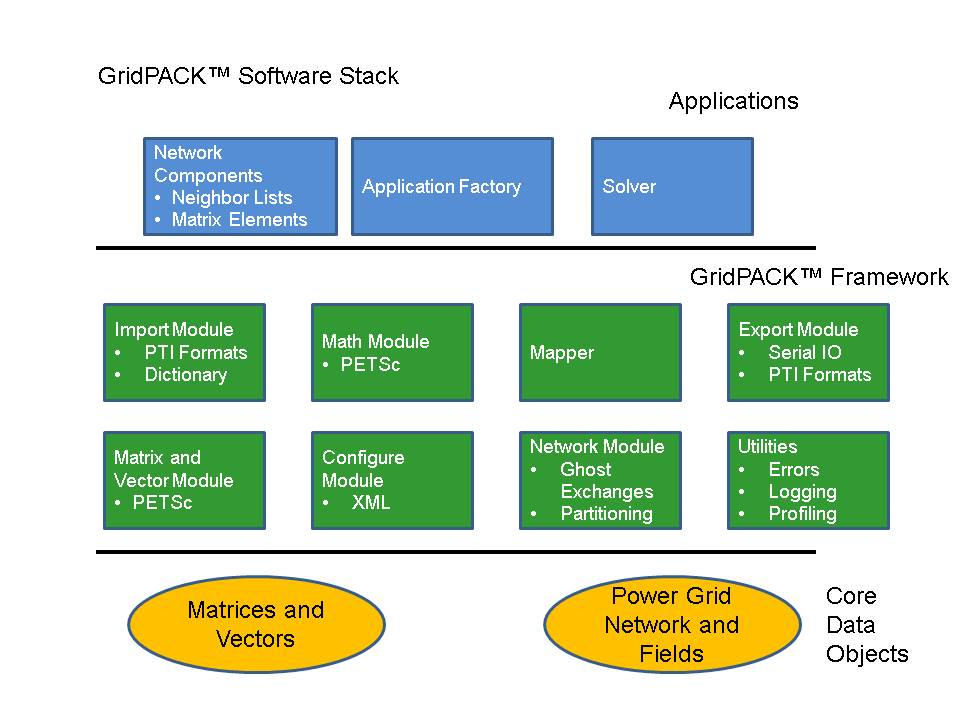
\includegraphics[width=5in,keepaspectratio=true]{./Fig1}
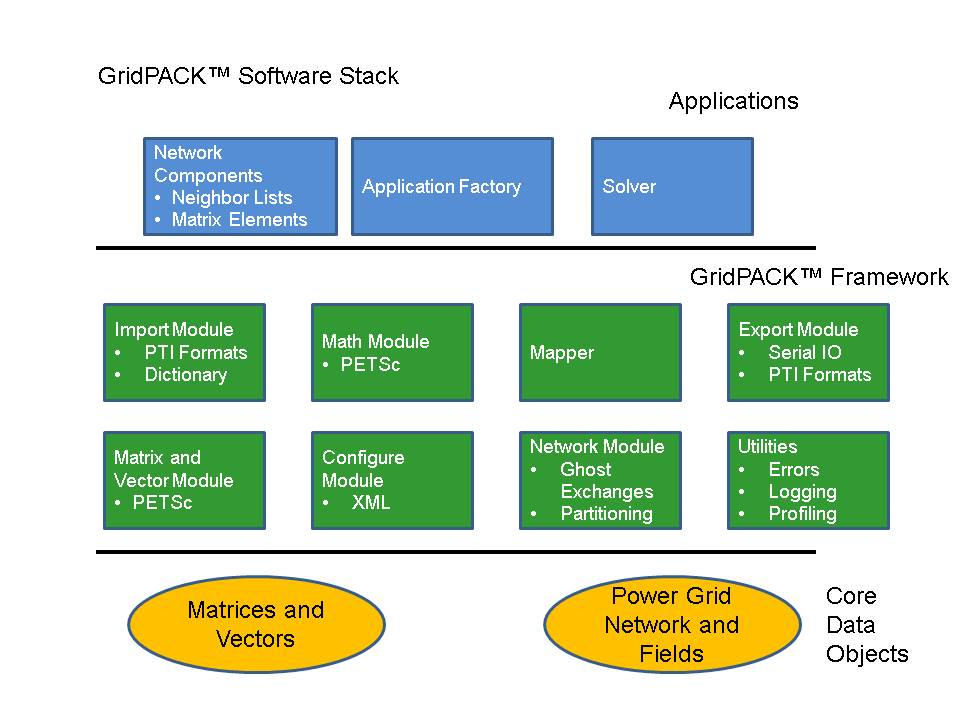
\includegraphics[width=3.5in,keepaspectratio=true]{./Fig1}
\caption{\label{stack} A schematic diagram of the GridPACK\texttrademark framework
software layers.
Yellow is used for core distributed data objects, green for framework components
and blue for application-specific components.}
\end{figure}
The application-independent modules (in green) have been separated from
the application specific modules (in blue). The goal has been to
hide as much of the complexity of parallel programming as possible into
generic functionality that could be used by multiple applications. A
particular focus has been the routines that require extensive communication
and/or algorithmic complexity. Successfully encapsulating these into
standalone modules that can be used across applications could dramatically
reduce the level of effort required to write power grid applications.

As shown in the figure, application developers will need to focus on
writing three sets of modules. The network components
contain the descriptions of the physics and/or
measurements that are associated with buses and branches in the power grid
network. The network factory is a module that initializes the grid components
on the network after the network is originally created by the import module. The
factory can also be used to implement other functions that manage interactions
between the network and the network components.  The solver is built out of
the math module and encapsulates the solution algorithm for the application.
Several parallel applications are currently under development using the
GridPACK\texttrademark and are expected to be completed shortly.

\section{Acknowledgments}
Funding for this work was provided by the U.S. Department of Energy's Office of
Electricity through its Advanced Grid Modeling Program.
Additional funding was provided by the Future Power Grid Initiative at Pacific
Northwest National Laboratory through the Laboratory Directed Research and
Development program.
Pacific Northwest National Laboratory is located in Richland, WA and is operated
by Battelle Memorial Institute under contract DE-AC05-76RLO1830 with the U.S.
Department of Energy. The authors would like to acknowledge insightful
discussions with Gilbert Bindewald at the Department of Energy and Dick Russell,
Jeff Dagle, and David Chassin at Pacific Northwest National Laboratory.

\bibliographystyle{abbrv}
\bibliography{gridpack}
\end{document}
